%%% File-Information {{{
%%% Filename: template_bericht.tex
%%% Purpose: lab report, technical report, project report
%%% Time-stamp: <2004-06-30 18:19:32 mp>
%%% Authors: The LaTeX@TUG-Team [http://latex.tugraz.at/]:
%%%          Karl Voit (vk), Michael Prokop (mp), Stefan Sollerer (ss)
%%% History:
%%%   20050914 (ss) correction of "backref=true" to "backref" due to hyperref documentation
%%%   20040630 (mp) added comments to foldmethod at end of file
%%%   20040625 (vk,ss) initial version
%%%
%%% Notes:
%%%
%%%
%%%
%%% }}}
%%%%%%%%%%%%%%%%%%%%%%%%%%%%%%%%%%%%%%%%%%%%%%%%%%%%%%%%%%%%%%%%%%%%%%%%%%%%%%%%
%%% main document {{{

\documentclass[
a4paper,     %% defines the paper size: a4paper (default), a5paper, letterpaper, ...
% landscape,   %% sets the orientation to landscape
% twoside,     %% changes to a two-page-layout (alternatively: oneside)
% twocolumn,   %% changes to a two-column-layout
% headsepline, %% add a horizontal line below the column title
% footsepline, %% add a horizontal line above the page footer
% titlepage,   %% only the titlepage (using titlepage-environment) appears on the first page (alternatively: notitlepage)
% parskip,     %% insert an empty line between two paragraphs (alternatively: halfparskip, ...)
% leqno,       %% equation numbers left (instead of right)
% fleqn,       %% equation left-justified (instead of centered)
% tablecaptionabove, %% captions of tables are above the tables (alternatively: tablecaptionbelow)
% draft,       %% produce only a draft version (mark lines that need manual edition and don't show graphics)
% 10pt         %% set default font size to 10 point
% 11pt         %% set default font size to 11 point
12pt         %% set default font size to 12 point
]{scrartcl}  %% article, see KOMA documentation (scrguide.dvi)

\newcommand{\sidebysidepic}[6]{
\begin{figure}[ht!]%
\begin{subfigure}{.5\textwidth}%
  \centering%
  \includegraphics[width=.8\linewidth]{#1}%
  \caption{#2}%
\end{subfigure}%
\begin{subfigure}{.5\textwidth}%
  \centering%
  \includegraphics[width=.8\linewidth]{#3}%
  \caption{#4}%
\end{subfigure}%
\caption{#5}%
\label{#6}%
\end{figure}%
}

%%%%%%%%%%%%%%%%%%%%%%%%%%%%%%%%%%%%%%%%%%%%%%%%%%%%%%%%%%%%%%%%%%%%%%%%%%%%%%%%
%%%
%%% packages
%%%

%%%
%%% encoding and language set
%%%

%%% ngerman: language set to new-german
\usepackage[english]{babel} 
\usepackage{tocloft}
\usepackage{subcaption}

%%% babel: language set (can cause some conflicts with package ngerman)
%%%        use it only for multi-language documents or non-german ones
%\usepackage[ngerman]{babel}

%%% inputenc: coding of german special characters
\usepackage[latin1]{inputenc}

%%% fontenc, ae, aecompl: coding of characters in PDF documents
\usepackage[T1]{fontenc}
\usepackage{ae,aecompl}

%%%
%%% technical packages
%%%

%%% amsmath, amssymb, amstext: support for mathematics
%\usepackage{amsmath,amssymb,amstext}

%%% psfrag: replace PostScript fonts
\usepackage{psfrag}

%%% listings: include programming code
%\usepackage{listings}

%%% units: technical units
%\usepackage{units}

%%%
%%% layout
%%%

%%% scrpage2: KOMA heading and footer
%%% Note: if you don't use this package, please remove 
%%%       \pagestyle{scrheadings} and corresponding settings
%%%       below too.
\usepackage[automark]{scrpage2}


%%%
%%% PDF
%%%

\usepackage{ifpdf}

%%% Should be LAST usepackage-call!
%%% For docu on that, see reference on package ``hyperref''
\ifpdf%   (definitions for using pdflatex instead of latex)

  %%% graphicx: support for graphics
  \usepackage[pdftex]{graphicx}

  \pdfcompresslevel=9

  %%% hyperref (hyperlinks in PDF): for more options or more detailed
  %%%          explanations, see the documentation of the hyperref-package
  \usepackage[%
    %%% general options
    %pdftex=true,      %% sets up hyperref for use with the pdftex program
    %plainpages=false, %% set it to false, if pdflatex complains: ``destination with same identifier already exists''
    %
    %%% extension options
    backref,      %% adds a backlink text to the end of each item in the bibliography
    pagebackref=false, %% if true, creates backward references as a list of page numbers in the bibliography
    colorlinks=false,   %% turn on colored links (true is better for on-screen reading, false is better for printout versions)
    %
    %%% PDF-specific display options
    bookmarks=true,          %% if true, generate PDF bookmarks (requires two passes of pdflatex)
    bookmarksopen=false,     %% if true, show all PDF bookmarks expanded
    bookmarksnumbered=false, %% if true, add the section numbers to the bookmarks
    %pdfstartpage={1},        %% determines, on which page the PDF file is opened
    pdfpagemode=UseNone         %% None, UseOutlines (=show bookmarks), UseThumbs (show thumbnails), FullScreen
  ]{hyperref}


  %%% provide all graphics (also) in this format, so you don't have
  %%% to add the file extensions to the \includegraphics-command
  %%% and/or you don't have to distinguish between generating
  %%% dvi/ps (through latex) and pdf (through pdflatex)
  \DeclareGraphicsExtensions{.pdf}

\else %else   (definitions for using latex instead of pdflatex)

  \usepackage[dvips]{graphicx}

  \DeclareGraphicsExtensions{.eps}

  \usepackage[%
    dvips,           %% sets up hyperref for use with the dvips driver
    colorlinks=false %% better for printout version; almost every hyperref-extension is eliminated by using dvips
  ]{hyperref}

\fi


%%% sets the PDF-Information options
%%% (see fields in Acrobat Reader: ``File -> Document properties -> Summary'')
%%% Note: this method is better than as options of the hyperref-package (options are expanded correctly)
\hypersetup{
  pdftitle={Image Based Measurement Laboratory 1}, %%
  pdfauthor={Filzmaier Josef, Michael Sieberer}, %%
  pdfsubject={Image Stitching, Auto-Focus, Sensor Dynamics, Perspective invariants}, %%
  pdfcreator={Accomplished with LaTeX2e and pdfLaTeX with hyperref-package.}, %% 
  pdfproducer={}, %%
  pdfkeywords={} %%
}


%%%%%%%%%%%%%%%%%%%%%%%%%%%%%%%%%%%%%%%%%%%%%%%%%%%%%%%%%%%%%%%%%%%%%%%%%%%%%%%%
%%%
%%% user defined commands
%%%

%%% \mygraphics{}{}{}
%% usage:   \mygraphics{width}{filename_without_extension}{caption}
%% example: \mygraphics{0.7\textwidth}{rolling_grandma}{This is my grandmother on inlinescates}
%% requires: package graphicx
%% provides: including centered pictures/graphics with a boldfaced caption below
%% 
\newcommand{\mygraphics}[3]{
  \begin{center}
    \includegraphics[width=#1, keepaspectratio=true]{#2} \\
    \textbf{#3}
  \end{center}
}

%%%%%%%%%%%%%%%%%%%%%%%%%%%%%%%%%%%%%%%%%%%%%%%%%%%%%%%%%%%%%%%%%%%%%%%%%%%%%%%%
%%%
%%% define the titlepage
%%%

% \subject{}   %% subject which appears above titlehead
% \titlehead{} %% special heading for the titlepage

%%% title
\title{Image Based Measurement Laboratory\\\vspace{1cm}\Large{Lab1 - Uncalibrated Sensors}}

%%% author(s)
\author{Filzmaier Josef (1030462) \and
Michael Sieberer (1531366)}

%%% date
\date{Graz, am \today{}}

% \publishers{}

% \thanks{} %% use it instead of footnotes (only on titlepage)

% \dedication{} %% generates a dedication-page after titlepage


%%% uncomment following lines, if you want to:
%%% reuse the maketitle-entries for hyperref-setup
%\newcommand\org@maketitle{}
%\let\org@maketitle\maketitle
%\def\maketitle{%
%  \hypersetup{
%    pdftitle={\@title},
%    pdfauthor={\@author}
%    pdfsubject={\@subject}
%  }%
%  \org@maketitle
%}


%%%%%%%%%%%%%%%%%%%%%%%%%%%%%%%%%%%%%%%%%%%%%%%%%%%%%%%%%%%%%%%%%%%%%%%%%%%%%%%%
%%%
%%% set heading and footer
%%%

%%% scrheadings default: 
%%%      footer - middle: page number
\pagestyle{scrheadings}

%%% user specific
%%% usage:
%%% \position[heading/footer for the titlepage]{heading/footer for the rest of the document}

%%% heading - left
% \ihead[]{}

%%% heading - center
% \chead[]{}

%%% heading - right
% \ohead[]{}

%%% footer - left
% \ifoot[]{}

%%% footer - center
% \cfoot[]{}

%%% footer - right
% \ofoot[]{}

\renewcommand*{\thesection}{Exercise~\arabic{section}:}
\renewcommand*{\thesubsection}{\arabic{section}.\arabic{subsection}}
\setlength{\cftsecnumwidth}{6.0em}
\setlength\parindent{0pt}

%%%%%%%%%%%%%%%%%%%%%%%%%%%%%%%%%%%%%%%%%%%%%%%%%%%%%%%%%%%%%%%%%%%%%%%%%%%%%%%%
%%%
%%% begin document
%%%

\begin{document}

% \pagenumbering{roman} %% small roman page numbers

%%% include the title
% \thispagestyle{empty}  %% no header/footer (only) on this page
 \maketitle

%%% start a new page and display the table of contents
 \tableofcontents
 \newpage

\section{Image stitching}

\subsection{Problem statement}

Shoot two consecutive pictures containing the target and combine them into a single image. Make use of the
target to define point correspondences, which were used to calculate an according homography. The MATLAB
function \texttt{PanoramaStiching.m} is provided and displays the stitched image given the two images and extracted
correspondences.

\begin{itemize}
 \item Try different numbers of point correspondences.
 \item Vary the distance between selected corners (i.e. select corners near each border of the target. Next time choose four corners placed around a single square).
 \item Why are some correspondences better than others? How can certain differences along the line of intersection be explained? Compare and discuss your results.
\end{itemize}

\subsection{Solution}

Two images from two different perspectives containing a target are taken with two different cameras.
Figure \ref{fig:photo12.5mm} shows the photos taken with a focus length of $12.5mm$ while Figure \ref{fig:photo6.5mm} shows the photos taken with a focus length of $6.5mm$.
The target is the chess board seen in both pictures of each focal length.

\sidebysidepic{./Bildg_Messtechnik_Lab/PanoramaStitching/images/image_1.png}
{First perspective}
{./Bildg_Messtechnik_Lab/PanoramaStitching/images/image_2.png}
{Second perspective}
{Images capturing target from different perspectives with $12.5mm$ focal length}
{fig:photo12.5mm}

\sidebysidepic{./Bildg_Messtechnik_Lab/PanoramaStitching/images/image_b1.png}
{First perspective}
{./Bildg_Messtechnik_Lab/PanoramaStitching/images/image_b2.png}
{Second perspective}
{Images capturing target from different perspectives with $6.5mm$ focal length}
{fig:photo6.5mm}

Corners within the chess board were chosen as unique locations to stitch the two images.
At first four unique image locations within the target are chosen in the first image.
These locations are mapped onto the second image with variyng accuracy.
Several scenarios are evaluated:
\subsubsection{All points are corresponding within the target over a large area}

\begin{figure}[ht!]
 \centering
 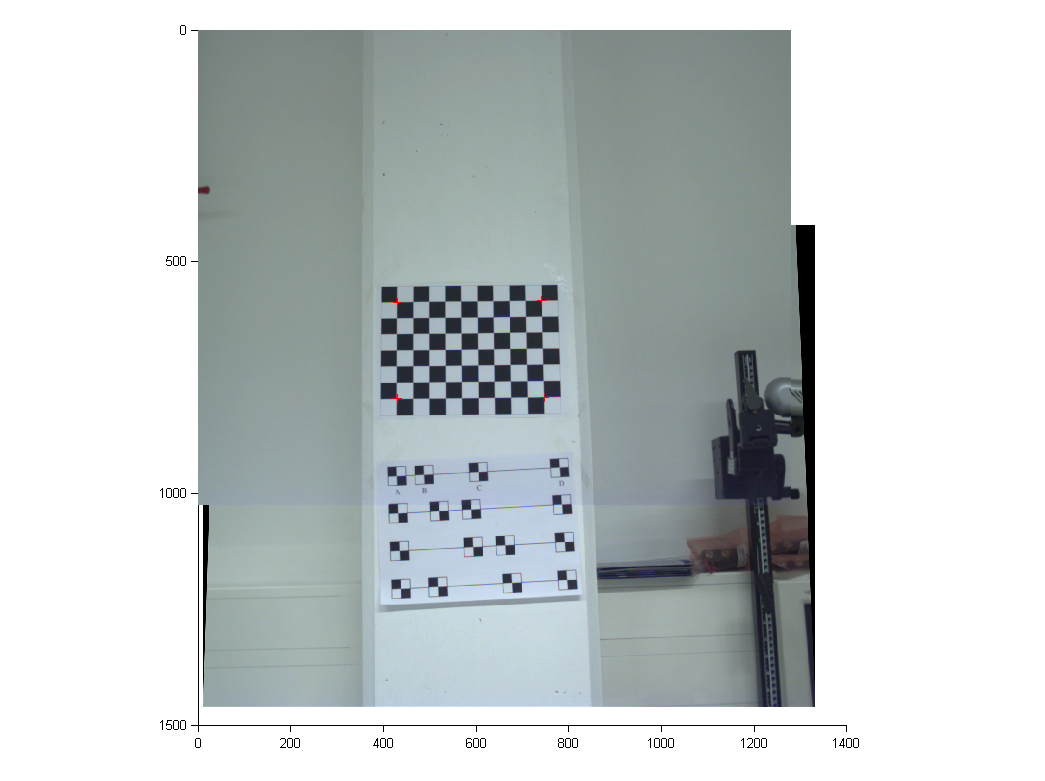
\includegraphics[scale=0.5]{./Bildg_Messtechnik_Lab/PanoramaStitching/fig1.png}
 \label{fig:largeareastitch12.5mm}
 \caption{Stitched image with points chosen over large area ($12.5mm$)}
\end{figure}

\begin{figure}[ht!]
 \centering
 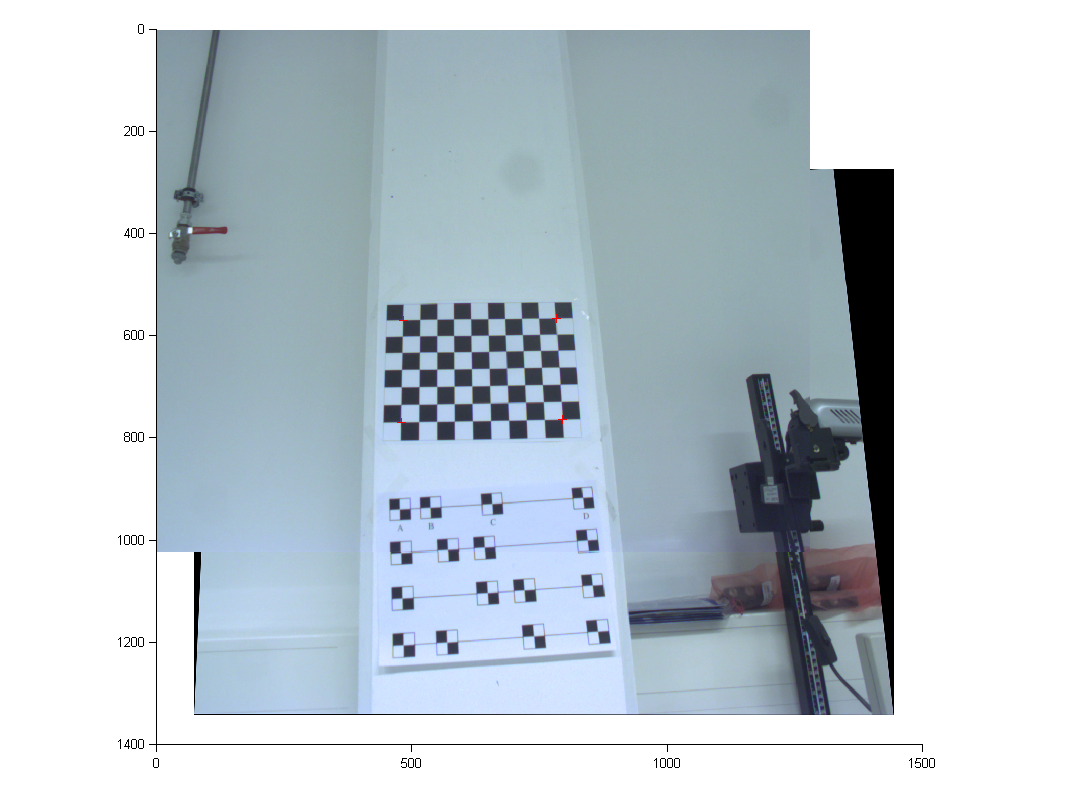
\includegraphics[scale=0.5]{./Bildg_Messtechnik_Lab/PanoramaStitching/figb1.png}
 \label{fig:largeareastitch6.5mm}
 \caption{Stitched image with points chosen over large area ($6.5mm$)}
\end{figure}

\subsubsection{All points are corresponding within the target over a small area}

\begin{figure}[ht!]
 \centering
 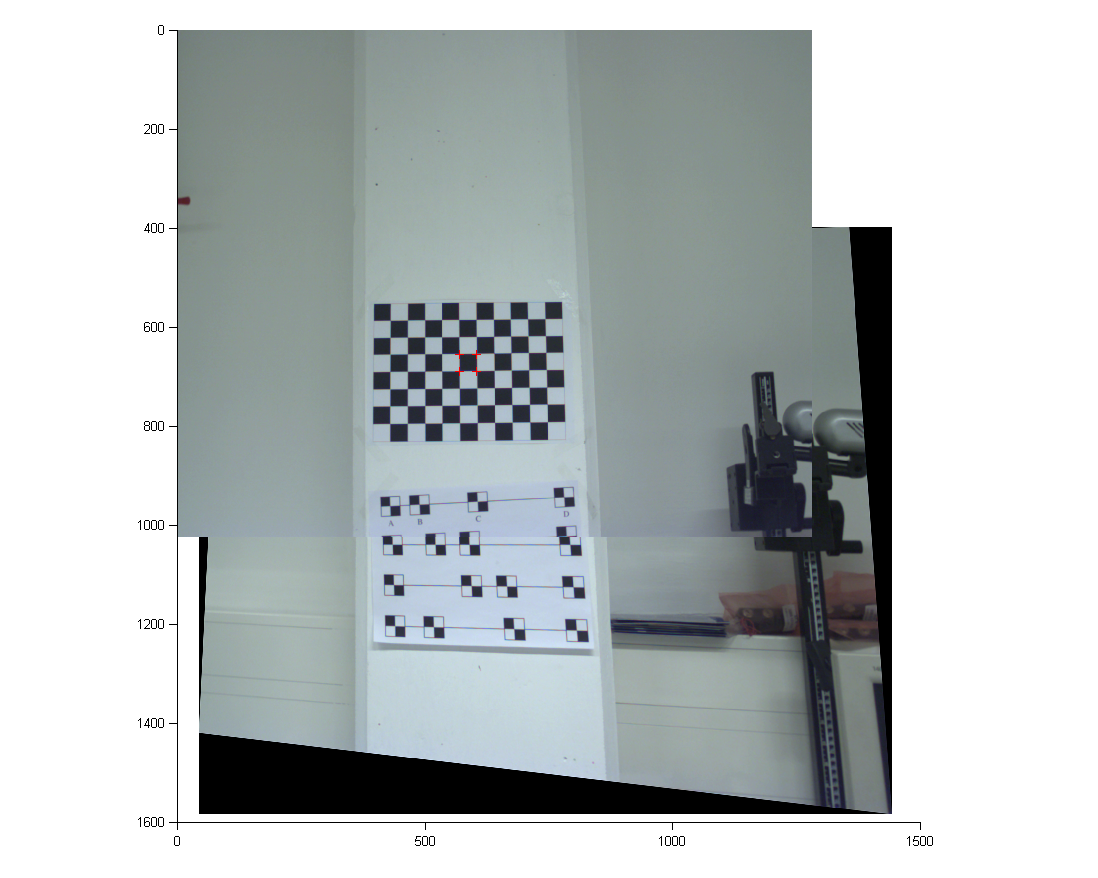
\includegraphics[scale=0.5]{./Bildg_Messtechnik_Lab/PanoramaStitching/fig2.png}
 \label{fig:smallareastitch12.5mm}
 \caption{Stitched image with points chosen over small area ($12.5mm$)}
\end{figure}

\begin{figure}[ht!]
 \centering
 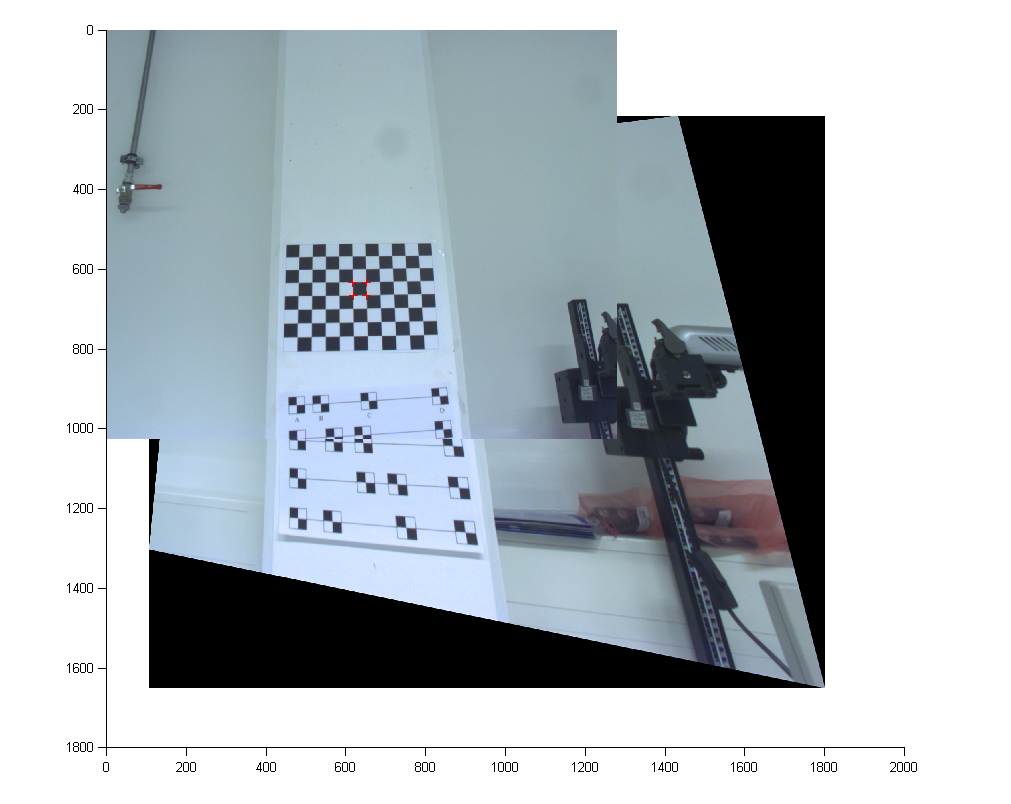
\includegraphics[scale=0.5]{./Bildg_Messtechnik_Lab/PanoramaStitching/figb2.png}
 \label{fig:smallareastitch6.5mm}
 \caption{Stitched image with points chosen over small area ($6.5mm$)}
\end{figure}

\subsubsection{One of the points is chosen differently in image two}

\begin{figure}[ht!]
 \centering
 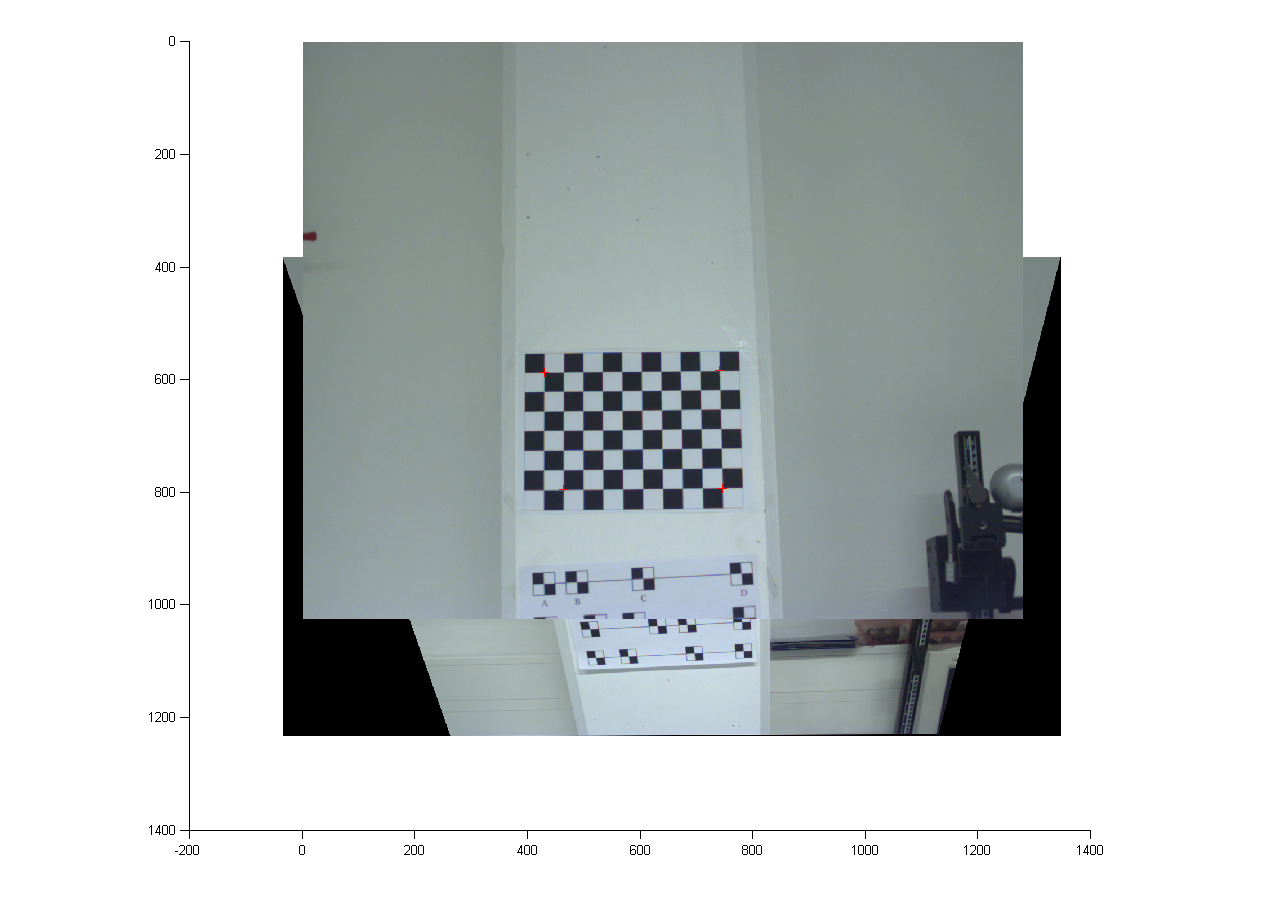
\includegraphics[scale=0.5]{./Bildg_Messtechnik_Lab/PanoramaStitching/fig3.png}
 \label{fig:differentareastitch12.5mm}
 \caption{Stitched image with points chosen over large area ($12.5mm$)}
\end{figure}

\begin{figure}[ht!]
 \centering
 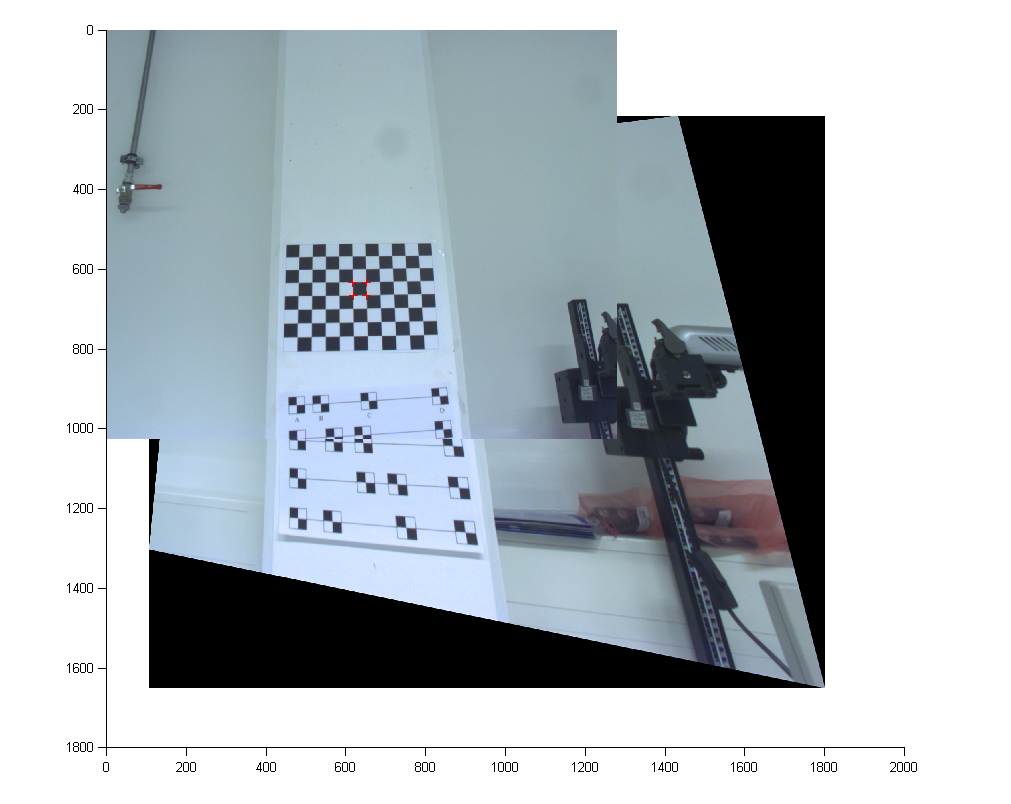
\includegraphics[scale=0.5]{./Bildg_Messtechnik_Lab/PanoramaStitching/figb2.png}
 \label{fig:differentareastitch6.5mm}
 \caption{Stitched image with points chosen over large area ($6.5mm$)}
\end{figure}

\subsubsection{All points are on one line except for one}
\subsubsection{An arbitrary constellation of corresponding points}

\pagebreak

\section{Auto Focus}

In this exercise we had to take a sequence of $N=10$ images with linearly varying focus and the determine which image has the best focus option.
In order to solve this task we implemented the following idea:

\begin{itemize}
 \item Convert the colored image to the corresponding grey value image
 \item Calculate the histogram of the grey value image
 \item Sort the histogram values decreasingly
 \item Sum up the first $1000$ elements of the sorted histogram and normalize
\end{itemize}

\pagebreak

\section{Sensor Dynamics}

In this exercise a black and white colored disk with an embedded EMT logo is spun up using an electronic motor.
The goal is to take a photo of the EMT logo while the disk is spinning.
This is done using a LED flashlight which is triggered by a rotation sensor and synchronously flashes the disk.
Therefore the logo is perceived static because the light highlights the disk always when the logo is at the same place.

\subsection{Global Shutter}

A global shutter camera measures light intensity with all pixel sensors at the same point in time.

\subsection{Rolling Shutter}

A rolling shutter camera measures light intensity line by line.
This can cause certain artifacts with fast moving objects.

\pagebreak
\section{Perspective Invariants}

In this exercise we take a photo of an prepared image with four points which have a certain distance to each other.
The points are prepared to easily be detected by a cornerMark function which is given in the framework.
Two different cameras with focal lenth of $4.3mm$ and $12.5mm$ were used.\\

\noindent
The claim to verify is that formula \ref{eq:cross_ratio} is independent of the perspective the picture is taken from as well as independent of the used focal length.

\begin{equation}
 CR_{A,B,C,D} = \frac{\overline{AC}}{\overline{BC}} : \frac{\overline{AD}}{\overline{BD}}
 \label{eq:cross_ratio}
\end{equation}

\subsection{Measuring by hand}

\begin{minipage}{0.48\textwidth}
  $$\overline{AB} = 42mm$$
  $$\overline{BC} = 82mm$$
  $$\overline{CD} = 123mm$$
\end{minipage}
\begin{minipage}{0.48\textwidth}
  $$\overline{AC} = 123mm$$
  $$\overline{BD} = 205mm$$
  $$\overline{AD} = 246mm$$
\end{minipage}

\hspace{0.5mm}

$$CR_{A,B,C,D} = \frac{\overline{AC}}{\overline{BC}} : \frac{\overline{AD}}{\overline{BD}} = \frac{123mm}{82mm} : \frac{246mm}{205mm} = 1.25$$

\subsection{Measuring using the cornerMark Matlab algorithm}



%%%
%%% end main document
%%%
%%%%%%%%%%%%%%%%%%%%%%%%%%%%%%%%%%%%%%%%%%%%%%%%%%%%%%%%%%%%%%%%%%%%%%%%%%%%%%%%

% \appendix  %% include it, if something (bibliography, index, ...) follows below

%%%%%%%%%%%%%%%%%%%%%%%%%%%%%%%%%%%%%%%%%%%%%%%%%%%%%%%%%%%%%%%%%%%%%%%%%%%%%%%%
%%%
%%% bibliography
%%%
%%% available styles: abbrv, acm, alpha, apalike, ieeetr, plain, siam, unsrt
%%%
% \bibliographystyle{plain}

%%% name of the bibliography file without .bib
%%% e.g.: literatur.bib -> \bibliography{literatur}
% \bibliography{FIXXME}

\end{document}
%%% }}}
%%% END OF FILE
%%%%%%%%%%%%%%%%%%%%%%%%%%%%%%%%%%%%%%%%%%%%%%%%%%%%%%%%%%%%%%%%%%%%%%%%%%%%%%%%
%%% Notice!
%%% This file uses the outline-mode of emacs and the foldmethod of Vim.
%%% Press 'zi' to unfold the file in Vim.
%%% See ':help folding' for more information.
%%%%%%%%%%%%%%%%%%%%%%%%%%%%%%%%%%%%%%%%%%%%%%%%%%%%%%%%%%%%%%%%%%%%%%%%%%%%%%%%
%% Local Variables:
%% mode: outline-minor
%% OPToutline-regexp: "%% .*"
%% OPTeval: (hide-body)
%% emerge-set-combine-versions-template: "%a\n%b\n"
%% End:
%% vim:foldmethod=marker
